\chapter{Deploy}
Once understood how create the server and generate the data to insert into it, the last phase is deploy the product.
\\ 
Before that what i've had to do is create a OCI image, from the Dockerfile, using the docker build, command.
\begin{figure}[h]
    \caption{Build and save the OCI image}
    \centering
    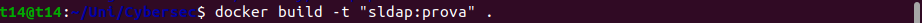
\includegraphics[width=15cm]{img/build.png}
    
\includegraphics[width=15cm]{img/save.png}
\end{figure}
\\
After that i can run the OCI image, as follow:
\begin{figure}[h]
    \caption{Load and run the server}
    \centering
    
\includegraphics[width=15cm]{img/load.png}
    
\includegraphics[width=15cm]{img/runb.png}
    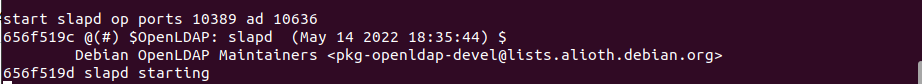
\includegraphics[width=15cm]{img/run.png}
\end{figure}
\\\\
Now everithing is ready and setted up, so a cybersecurity expert can download the image and run it with randomly generated data, that use a Ollama to generate them.
